\chapter{Languages}
\label{languages}
The preceding chapter described a representation for programs which is suitable for any language. To define a particular language in this framework involves defining three aspects of the language.

The \emp{abstract syntax} of the language defines what nodes may appear in a program, and in what relationship to each other. In \Meta, abstract syntax is defined by a program in the \keyword{grammar} language. The grammar program is first and foremost a specification which defines what programs are (syntactically) valid. 

Every language must have a \emp{semantics} that gives its programs meaning. 
%While there are a number of ways to specify semantics, or indeed to make use of languages and programs with only ill-defined semantics, a
A particularly economical way to give semantics is to define a minimal \emp{kernel} language and then define the remainder of the language in terms of reduction from an enriched syntax to the kernel syntax. Concretely, when a grammar defines a node type, it may also define the semantics of the construct by means of a reduction to a more primitive construct. This approach is commonly used to \emp{define} languages, but not necessarily to implement them (see, e.g. Mozart \cite{mozart}). In \Meta, as in Lisp, this economical approach is opened up to the programmer---the same extension mechanism used to define the core language is available in all programs. The example of Lisp (particularly, Scheme \cite{scheme}) shows this to be a workable strategy, so the experimental question is how well it applies in this new setting.

Thus a \Meta\ grammar defines a language's syntax and gives a semantics for programs in that language in terms of the kernel language programs they reduce to. A second kind of semantics that may be desired is \emp{static semantics}, that is, specification of additional constraints on valid programs including anything from proper scoping of references to a type system. These constraints could also be specified in a grammar language, but \Meta\ does not currently support such declarations. 
%\temp{However, some of the constraints that might normally be considered part of a language's static semantics are taken care of at a lower level in \Meta. For example, there is no need to test for the presence of a variable declaration; in Meta, a variable reference is represented as a reference node which is constrained to refer to a node somewhere in the program; the editor ...}

With abstract syntax and semantics taken care of, both the Lisper and the Programming Language Theorist have all they need and will go happily on their ways. However, we would like to go further than that, so one more element is needed. \emp{Concrete syntax} is what the user reads and writes. The goal is to take advantage of the new approach to do things with concrete syntax that are impractical or impossible to do with textual source code. In \Meta, the concrete syntax of each type of node is given as a reduction to a \emp{presentation language}.

%
% Grammars
%
\section{Grammars}
\label{grammars}
A grammar defines all three aspects of a language. The abstract syntax is defined \emp{prescriptively}, by identifying the subset of all possible programs which are valid. Both the semantics and concrete syntax are defined \emp{operationally}, as declarations of what reduced program and what visual representation will be derived from each source node.

\subsection{Abstract Syntax}
A program is \emp{valid} with respect to a \emp{grammar} if all of its nodes' types, values, and references comply with the constraints imposed by the grammar. For each node type, a grammar specifies:
\begin{enumerate}
\item Zero or more \emp{abstract types}, which are types for which the type being introduced is a \emp{sub-type}.
%\item Whether the node's value should be an boolean, integer, string, sequence, or map.
%\item For an integer-valued node, a range of legal values.
\item For a sequence node, the expected number and (abstract) type of child nodes.
\item For a map node, the expected attributes and the (abstract) types of nodes that may inhabit each of them.
\item When a child/attribute is a reference, the expected (abstract) type of the referenced node.
\end{enumerate}

Abstract types lend some modularity to the grammar. A new subtype of any abstract type can be introduced later without changing any existing definition, and nodes with the new type can appear as children of nodes which were declared using the abstract type. Figure \ref{fig-attrs} shows the declaration of a hypothetical node type \keyword{pow}, for expressions raising some runtime value to a fixed integer power. \keyword{pow} is an instance of the abstract type \keyword{expr}. To be valid, a \keyword{pow} node must have an attribute \keyword{e}, containing a node whose type is an instance of \keyword{expr}, and another attribute \keyword{n}, an integer. So far, this declaration mimics the way you might define a similar node as an algebraic data type in a functional language such as Haskell or ML.

\begin{figure}
	\centering

	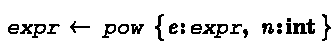
\includegraphics[scale=1.0]{src/image/pow.pdf}	
%	\texttt{expr} $\leftarrow$ \texttt{pow} \{ $e$ : \texttt{expr}, $n$ : \keyword{int} \}
	
	\caption{A simple node declaration.}
	\label{fig-attrs}
\end{figure}

Note that all the grammar constraints except the constraint on the types of referenced nodes are local in the sense described earlier---checking them requires inspecting only a single node and its immediate children. Checking the types of referenced nodes requires being able to inquire about the type of a node which may be anywhere in the program. However, this information is easily extracted up front to a map of types for all nodes in the tree, so this one non-local check seems to be worth including in the standard checker.

A grammar so-defined is not capable of specifying every interesting property of a language. That is, not every syntactically valid program is correct. Depending on the nature of the language being defined, additional, more ambitious specifications can define additional properties (e.g.\ static semantics). The abstract syntax is meant to be an easily-defined first step, and to provide the information needed by the editor to provide support for editing programs which use arbitrary new node types.


\subsection{Reductions}
In addition to defining what programs are syntactically valid, a grammar provides a definition of concrete syntax via a \emp{display} reduction and of semantics via an \emp{expand} reduction. Either or both reductions may be present in a declaration. These reductions are code fragments which are used to construct reduction functions (see section \ref{reduction}) which take a program in the source language defined by the grammar and reduce it to a derived program. Using a meta-programming approach, the reductions are economical and simple to define, but the full host language is available for use in reductions when needed.

\begin{figure}[t]
	\centering
	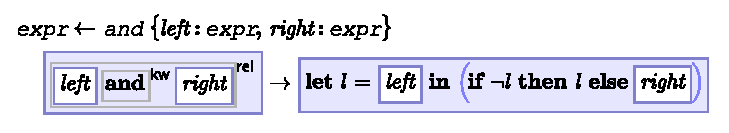
\includegraphics[scale=0.8]{src/image/and.pdf}
		
	\caption{The \keyword{or} node of the core language, including reductions.}
	\label{fig-and}
\end{figure}

A display reduction is always present and reduces a source node to a presentation language node (often the root of a sub-tree containing several presentation language nodes). On the lower left in Figure \ref{fig-and} is the display reduction for \keyword{or} nodes, which arranges the left and right children of the node into horizontal sequence, separated by the keyword ``or.''

An expand reduction is used to reduce a node in preparation for evaluation or execution, and therefore defines the semantics of the node. The result of this reduction is a node in the \emp{target language}, or else a node that will itself be reduced, eventually to a target language node. The declaration of a node type does not provide a expand reduction if the node is part of a target (kernel) language. On the lower right in Figure~\ref{fig-and} is the expand reduction, which defines the behavior of the \keyword{or} construct in terms of kernel language constructs: it evaluates the left argument and yields the value if it is not \keyword{false}, otherwise it evaluates the right argument and yields that value. This kind of short-circuiting evaluation returning the first ``true'' value is a common way of implementing the logical ``or'' operator in scripting languages \cite{javascript}\cite{clojure-and}\cite{python-and}.

It is easy to define a reduction that fails to terminate (for instance by producing a node of the same type), or which ``blows up'' (by producing a larger, but no more reduced, node). The usual approaches to proving termination of recursive algorithms apply. In any case, once language definition is part of the development process, it should no longer be so surprising that problems can arise at that level. Because you are your own language vendor, you can simply fix it; it's not like finding a bug in your C++ compiler, which you may have no capability to fix.

Thus the abstract syntax, semantics, and concrete syntax of every derived language construct are defined together in a simple, declarative style. Each construct is self-documenting; any use of a new construct can always be expanded (manually or automatically) to the equivalent reduced program.


%
% Kernel languages:
%

\section{Kernel Languages}
\label{kernel}
A \emp{kernel language} is one whose nodes have some fixed, pre-defined semantics (typically, they can be interpreted, yielding some specified result with some specified side effects). A complete language is built by \emp{extending} a kernel language with additional nodes whose semantics is defined in terms of reduction to (ultimately) the kernel language.

Any language can act as a kernel language in \Meta. If the kernel language is of a more conventional type, say Java, all the constructs of that language have to be defined as primitives. Additional constructs could then be defined via reduction to ordinary Java syntax. After reduction, the target program would be processed by a Java compiler to produce an executable. Thus a language like Java is a suitable kernel language, but hardly a convenient one.

I designed the \Meta's \emp{host kernel language} to be much simpler to implement and use. The host kernel language is designed to be:
\begin{enumerate}
\item Minimal, but sufficient to define a general-purpose language via extensions.
\item A meta-language, able to consume and produce nodes.
\item A ``functional'' language, operating naturally on immutable nodes and trees.
\item Easily implemented and easily integrated with existing software.
\end{enumerate}

These characteristics make the host kernel language---and the core language built on top of it---ideal for implementing \Meta\ itself. For example the reductions themselves are written in it. I describe the host language in detail in section \ref{host}.

%The idea of a very minimal kernel language with a core language built on top of it is of course inspired by the Lisp family of languages. In particular, in Scheme\cite{scheme}, only a handful of \emp{special forms} are pre-defined, and all other language constructs are defined ``in the language'' in terms of macros which expand into the special forms. A similar approach is used for more didactic purposes in Mozart\cite{mozart}, at least in \emp{defining} the language, although it isn't clear that the implementation actually works this way.


%
% Presentation languages:
%

\section{Presentation Languages}
\label{expr}
The nodes of a \emp{presentation} language cast program elements in visual terms. A presentation language should be independent of the particular syntax of any one language, but might be suited to a particular family of related languages. Crucially, the presentation language must be flexible enough to represent any conceivable construct that might be added to the source language. This is achieved by providing composable elements in the presentation language that can be combined in new ways to create new concrete syntax. In \Meta, a single presentation language is currently implemented.

\subsection{The \textit{\keyword{expr}} Presentation Language}

\Meta's \keyword{expr} presentation language is well-suited to representing the expressions that make up the declarative portion of a typical modern programming language in the usual way, except that it provides more typographically-rich elements. It can also reproduce much of the familiar notation of algebraic expressions. 

An \keyword{expr} program is represented internally as a tree made up of \emp{box} nodes. Each box node occupies a rectangular area of the rendering surface and always encloses the areas occupied by any child boxes, although this structure is not visible to the user, who sees a familiar layout of keywords, operators, and other textual elements. Several kinds of boxes are available in \keyword{expr}.

An \emp{atom} is a box that renders a sequence of characters and/or symbols using the normal spacing for text. Several types of atoms are available, each conveying what kind of entity the characters are meant to represent. When atoms are reduced to lower-level nodes, a distinctive typographical treatment is applied to each, as shown in Table~\ref{tab-atoms}. The set of atom types is meant to be easily expanded to serve the needs of any conceivable source language. The total number of types in any one language is probably limited to a dozen or so, and many are common across languages. Therefore I conjecture that the universe of useful atom types is not much larger than what \keyword{expr} currently provides. When a new type is needed, the effort to add it is typically small (most simply specify a font and/or face), 


\begin{table}

	\begin{center}
	\begin{tabular}{llll}
	Type & Treatment & Examples & Typical use
	\\
	\hline
	\keyword{keyword}
	 & boldface
	 & \keyword{true}
	 & fixed language syntax
	\\ & & \keyword{if} &   % Ugly hack! how to do proper multi-line cells in tabular env.?
	\\
	\hline
	\keyword{var}
	 & italic
	 & $x$
	 & names (user-provided or generated)
	\\ & & $g$ & 
	\\ & & $\mathit{fib}$ & 
	\\
	\hline
	\keyword{num}
	 & \textit{none}
	 & 1
	 & numerical literals
	\\ & & 2.0 & 
	\\ & & 3,000 & 
	\\
	\hline
	\keyword{string}
	 & sans serif
	 & \textsf{abc} 
	 & character literals (note special
	\\
	 & & \textsf{Hello,\textvisiblespace world} &  % open box: \u2423
	  treatment of the space character)
	\\
	\hline
	\keyword{name}
	 & boldface, italic
	 & \textbf{\emp{a}}
	 & name literals
	\\ & & \textbf{\emp{foo}} & 
	\\
	\hline
	\keyword{mono}
	 & monospaced
	 & \texttt{nil}
	 & external references
	\\ & & \texttt{cons} & 
	\\
	\hline
	\keyword{prod}
	 & monospaced, italic
	 & \texttt{\emp{expr}}
	 & node types in grammars
	\\ & & \texttt{\emp{left}} & 
	\\
	\hline
	\keyword{symbol}
	 & \textit{none}
	 & $\to$
	 & mathematical symbols
	\\ & & $\in$ & 
	\\ & & $\sum$ & 
	\\
	\hline
	\end{tabular}
	\end{center}
	
	\vspace{6pt}
	Note: the actual character content of each type of atom is arbitrary, except \keyword{symbol}, which handles only a pre-defined set of available symbols.

	\caption{Types of atoms in the \keyword{expr} language.}
	\label{tab-atoms}
\end{table}

%\begin{figure}[t]
%  \begin{center}
%  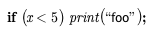
\includegraphics[scale=0.8]{src/image/if.png}  % 72dpi/0.8 = 88.75, actually
%  
%  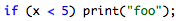
\includegraphics[scale=0.8]{src/image/if-text.png}
%  \end{center}
%  
%  A simple Java expression, rendered by \Meta\ and by a typical programmer's editor (TextMate), both at 90dpi. Note that the colored version is rendered using sub-pixel anti-aliasing, which looks better on screen than on the page.

%  \caption{Typographically-rich notation compared to ``syntax coloring.''}
%  \label{fig-syntax-coloring}
  
%\end{figure}

\emp{Composite} boxes contain child boxes which they arrange in a certain way. A \emp{sequence} is a horizontal arrangement of nodes separated by a certain amount of space. There are a handful of sequence types, each implying a certain amount of inter-node space. The amount of space is a visual indication of how tightly the sub-expression represented by the sequence binds, as I'll discuss in the next subsection. A \keyword{scripted} node contains a \emp{nucleus} and \emp{sub}- and/or \emp{super}-script nodes. \emp{Special signs} are similar to composites but also draw a glyph surrounding the child node(s). Examples are \keyword{radical} and \keyword{fraction}, used in particular mathematical contexts.

A \keyword{group} node draws a pair of grouping symbols around a content node. Available symbols include parentheses, various kinds of brackets, $\lfloor\mathit{floor}\rfloor$, $\lceil\mathit{ceiling}\rceil$, and $|\mathit{magnitude}|$. All these symbols expand vertically to visually surround their contents; this variation in size is aesthetically pleasing, but can also provide a visual cue which helps the reader to match up the paired symbols.

An \keyword{embed} node encloses its contents in a visual indication of being a separate unit, contained within the surrounding context. A \keyword{disembed} node has the opposite effect, showing its contents as being logically part of the outer level of code. These are used in the rendering of quotations, and have been seen already in the example reductions in Figure \ref{fig-and}.


\subsection{Expressive Power}

The diversity of atom types provides a measure of visual sophistication for programs, with a very small effort on the part of the language designer. Simply by identifying a visual style for each piece of syntax, some information about the meaning of each node is conveyed to the programmer. The particular treatment is meant to match the readability and high aesthetic standards of the pseudocode that might be found in a journal article or a good computer science textbook.\footnote{The reader can judge my success by inspecting any of the figures in this paper, most of which were captured directly from \Meta's editor as vector graphics.} The rendering of these fonts on screen at relatively low resolution of 100 dots per inch or less is not really optimal, but given the trend toward more dense displays (as of late 2010, laptop displays approaching 150 dpi are common and displays on handheld devices can be much higher than that), it is likely that acceptable rendering of multiple fonts even at small sizes will soon be quite achievable. In any case, the actual choice of how to present each type of atom is unrestricted; a more conventional approach would be to use just a few fonts and instead use color to distinguish different elements in the conventional ``syntax-highlighting'' manner \cite{lexx}. These issues have been explored heavily in the field of integrated development environments (IDEs), but few published studies seem to exist. One reference is Harward, et al \cite{insitu}.

Because the \keyword{expr} language preserves the hierarchical structure of expressions and specifies the visual layout of each sub-expression, it's possible for the system to identify cases where the nesting of expressions could lead to confusion, and to insert parentheses automatically in these cases. This is done \emp{after} the reduction of the program to the \keyword{expr} language, so it's applied consistently to any language construct, without special effort at the point of definition of a node. 

The \keyword{expr} language provides enough levels of spacing (four) to handle a moderately complex expression without parentheses. For example, in the expression
\begin{center}
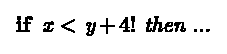
\includegraphics{src/image/space.pdf}
\end{center}  % too much space here (actually part of the pdf?), and an unfortunate page break, currently.
the factorial operator binds most tightly ($!$, no space), then addition is performed ($+$, with a thin space), then comparison ($<$, medium space), and finally the conditional (\keyword{if} \dots \keyword{then} \dots, thick space). Examples of how this works will be presented later.

A presentation language is concrete in that it represents the program as it is presented to the user, however it is somewhat abstracted from the details of rendering characters and pixels. The reduction from source to presentation language is therefore quite direct and simple. Once the program is reduced to the presentation language, lower-level processing takes care of the details of rendering. This lower-level processing is common to all languages using the same presentation language, and does not need to be extended in the typical course of using (and extending) a source language.

\keyword{expr} supports nested expressions well, and in combination with the lower-level presentation language (described in section \ref{view}) it can produce good results for some moderately complex programs if used with care. However to handle larger constructs such as classes or modules would raise layout problems that \keyword{expr} is not really intended to address. For example, how to handle indentation and when and how to break lines. Additional nodes could be added to \keyword{expr} to address these issues.

\Meta's presentation language, plus this kind of extension, should be able to implement most general purpose programming languages, and allow their syntaxes to be extended in new ways. With some additional features, it could also support new kinds of visualization and interaction for source code. For example, embedded images as in Sikuli\cite{sikuli}, or program elements that respond to clicks as in a typical structure editor.

Going further, to serve the needs of different kinds of languages, entirely different presentation languages could be defined, such as a ``flowing text'' language for documents, a ``grid'' language for spreadsheet-like programs, a ``flowchart'' language for state machines, data flow programs, and regular expressions, and so forth. These styles might call for an entirely new low-level presentation language and renderer, but the underlying framework of \Meta\ would be able to handle the jobs of defining languages, and validating and transforming the programs.

%
% Extending...
%

\section{Extending the Grammar Language}
The grammar language (section \ref{grammars}), host language (\ref{kernel}), and presentation language (\ref{expr}) work together to support the definition of new language constructs.
%\temp{When it's desirable to keep track of what source node gave rise to a given target node, the reduction can record the labels of each pair of source and target node, forming a kind of mapping between the parallel trees. For this to work, the reduction function needs to operate strictly on the single node it's given, and not reach into any child node. This in turn places some constraints on the way the source program is constructed: each node (along with any environment) must bear sufficient information to identify the correct reduction.}
A grammar is a \Meta\ program, so the same tools for syntax extension are available for use in grammars. The \keyword{grammar} language should be viewed as a starting point. It is meant to be general enough to define typical languages, to handle most common needs for defining syntax, and to serve as a kernel language for grammars.

As an example, consider the variety of 2-argument, infix operators that we may wish to define for the core language. If defined in terms of the kernel grammar language, each declaration will echo the definition of \keyword{or} shown in Figure \ref{fig-and}, varying only in the symbol used to represent the operator, and the name of a function to invoke. This kind of duplication is a clear opportunity for language extension, which you can do in \Meta\ by adding to the grammar for the grammar language itself. 

Figure \ref{fig-binary} shows the declaration of a new grammar node, \keyword{binaryNode}, with just four attributes for the parts of the declaration which are unique in each case: an optional documentation string, the name for the node being declared, the symbol which will represent the new operator for display purposes, and a function in the host language which implements the operation.

\begin{figure}[t]
	\centering
	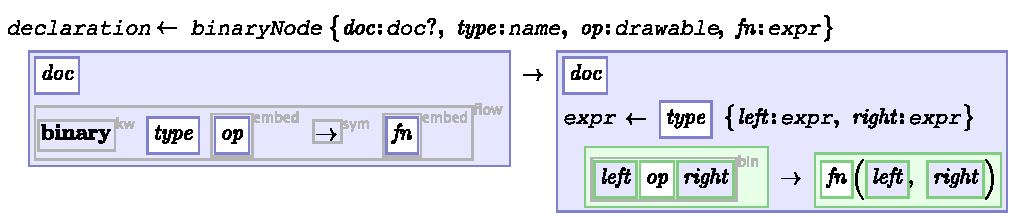
\includegraphics[scale=0.8]{src/image/binaryNode.pdf}

	\caption{Definition of \keyword{binaryNode} as an extension of the grammar syntax.}
	\label{fig-binary}
\end{figure}

\begin{figure}[t]
	\centering
	
	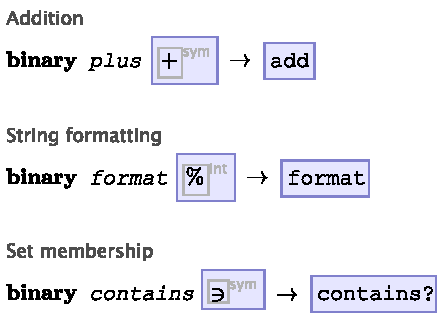
\includegraphics[scale=0.8]{src/image/binary.pdf}

  \caption{Some infix operators defined using \keyword{binaryNode}.}
  \label{fig-binary-examples}
\end{figure}

The display reduction (the blue, quoted box on the left) for these declarations mimics the regular node declaration syntax but omits the declaration of attributes and has just four editable elements. The expansion on the right is a quoted declaration which will be evaluated to produce an ordinary node declaration. Compared to the five nodes of the simplified declaration, the expanded declaration contains about 16 nodes. Like much syntax extension, the new node embodies the well-known goal of eliminating code duplication \cite{dry}. As seen in Figure~\ref{fig-binary-examples}, node types declarations using this new syntax are significantly simplified.

What's happening here is the concrete syntax and semantics of the new construct are given in the form of two small meta-programs. However, each reduction is presented in the rich syntax of its target language (the \keyword{expr} presentation language itself on the left, and the \keyword{grammar} language on the right), and the visual representation of quoted and un-quoted nodes gives the reductions the look of a simple template with ``holes'' for elements to be inserted. Thus the grammar language combines the power of meta-programming with a simple, understandable visual representation.

%\todo{Can this paragraph be turned into some kind of summary/wrap-up for the chapter as a whole?} A grammar (i.e.\ a program in the \keyword{grammar} language) consists of a collection of node type declarations (\keyword{grammar} nodes), each containing reductions (which are host language nodes). A \emp{display} reduction in turn contains quoted nodes in a presentation language (e.g.\ \keyword{expr}), while an \emp{expand} reduction quotes nodes in the target language (which may be the host language or some other target language). 

%\todo{where?} This is only the start; a grammar can define syntax for embedding subtrees in yet more languages, such as when a regular expression sub-language is added as an extension to a general-purpose language. This extensive embedding is the key to economy of expression in \Meta.\footnote{And it inspired the name \Meta. A grammar is a meta-language, so the grammar for grammars is a meta-meta-language. Warning: this kind of thing is fun when it works, but it can be a mind-twisting chore to get it bootstrapped.}
